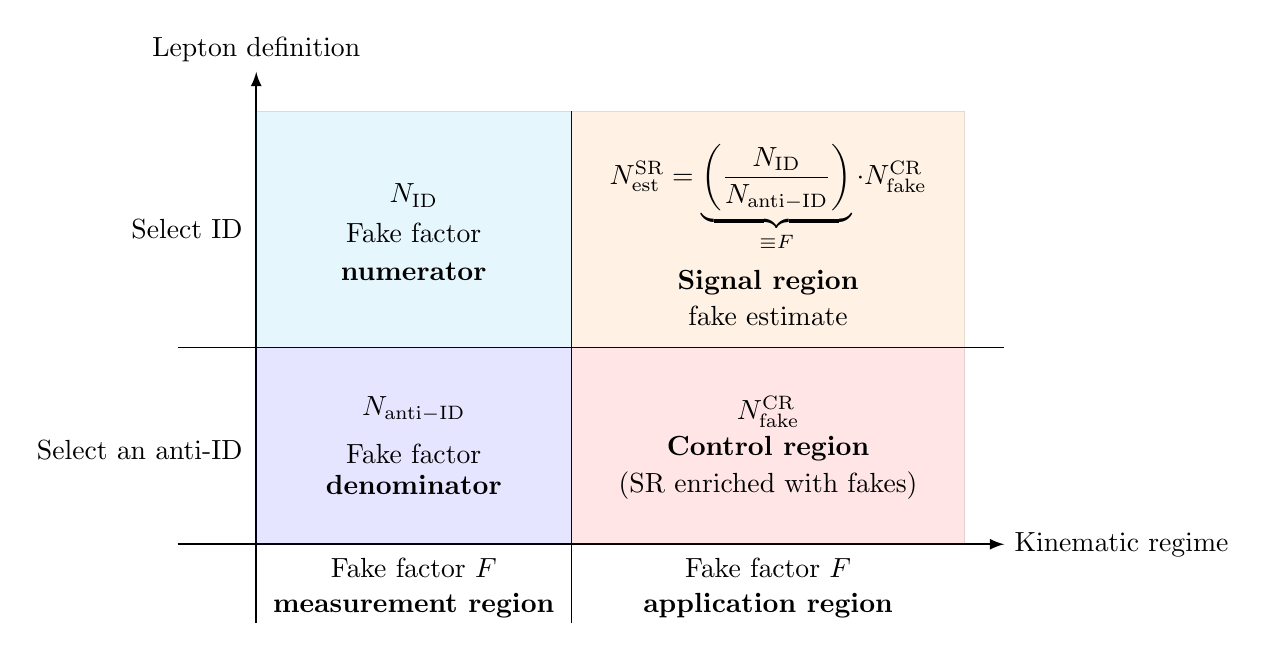
\begin{tikzpicture}
    
    % axes
    \draw [-latex, thick] (-1,0)--(9.5,0) node [right] {Kinematic regime};
    \draw [-latex, thick] (0,-1)--(0,6) node [above] {Lepton definition};
    
    % selection 
    \draw (4,-1) -- (4,5.5);
    \draw (-1,2.5) -- (9.5,2.5);
    
    % axis labels
    \node at (-0.05,4) [left] {Select ID};
    \node at (-0.05,1.2) [left] {Select an anti-ID};
    
    \node at (2,-0.05) [below] {Fake factor $F$};
    \node at (2,-0.5) [below] {\textbf{measurement region}};
    \node at (6.5,-0.05) [below] {Fake factor $F$};
    \node at (6.5,-0.5) [below] {\textbf{application region}};
    
    % boxes
    \draw [opacity=0.1, fill=blue] (0,0) -- (0,2.5)-- (4,2.5) -- (4,0) -- (0,0);
    \draw [opacity=0.1, fill=cyan] (0,2.5) -- (0,5.5)-- (4,5.5) -- (4,2.5) -- (0,2.5);
    \draw [opacity=0.1, fill=red] (4,0) -- (4,2.5)-- (9,2.5) -- (9,0) -- (4,0);
    \draw [opacity=0.1, fill=orange] (4,2.5) -- (4,5.5)-- (9,5.5) -- (9,2.5) -- (4,2.5);
    
    % box labels
    \node at (2,2) [below] {$N_\mathrm{anti-ID}$};
    \node at (2,1.4) [below] {Fake factor};
    \node at (2,1) [below] {\textbf{denominator}};
    
    \node at (2,4.7) [below] {$N_\mathrm{ID}$};
    \node at (2,4.2) [below] {Fake factor};
    \node at (2,3.7) [below] {\textbf{numerator}};
    
    \node at (6.5,5.2) [below] {$N^\mathrm{SR}_\mathrm{est} = \underbrace{\left(\displaystyle\frac{N_\mathrm{ID}}{N_\mathrm{anti-ID}}\right)}_{\equiv F}\cdot N^\mathrm{CR}_\mathrm{fake}$};
    \node at (6.5,3.6) [below] {\textbf{Signal region}};
    \node at (6.5,3.15) [below] {fake estimate};
    
    \node at (6.5,2) [below] {$N^\mathrm{CR}_\mathrm{fake}$};
    \node at (6.5,1.5) [below] {\textbf{Control region}};
    \node at (6.5,1.05) [below] {(SR enriched with fakes)};
    
\end{tikzpicture}
